\documentclass[tikz,border=2pt]{standalone}
\usetikzlibrary{arrows.meta,positioning,calc,shapes.geometric}
\usepackage{fontspec}
\setmainfont{TeX Gyre Termes}
\setsansfont{Roboto}
\begin{document}
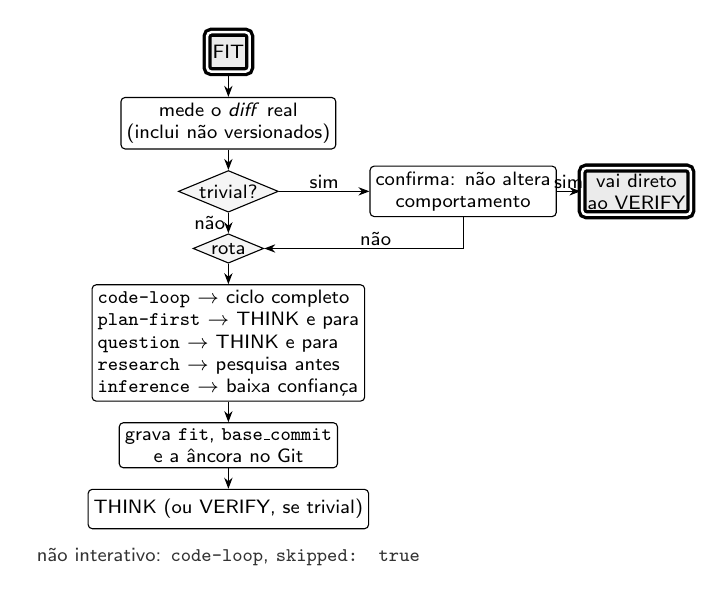
\begin{tikzpicture}[
  font=\sffamily\scriptsize,
  >={Stealth[length=4pt]},
  proc/.style={draw, thin, rounded corners=1.5pt, align=center, fill=white,
    minimum height=0.5cm, inner sep=2pt},
  exec/.style={proc, very thick, double distance=0.9pt, fill=black!8},
  dec/.style={draw, thin, diamond, aspect=2.4, align=center, fill=black!4,
    inner sep=0.5pt, font=\sffamily\scriptsize},
  nota/.style={font=\sffamily\scriptsize, align=center, text=black!80},
  lbl/.style={font=\sffamily\scriptsize, inner sep=1pt}
]
\node[exec] (fit) {FIT};
\node[proc, below=0.3cm of fit] (d) {mede o \textit{diff} real\\ (inclui não versionados)};
\node[dec, below=0.26cm of d] (t) {trivial?};
\node[dec, below=0.26cm of t] (r) {rota};
% ramo da direita: confirma -> atalho
\node[proc, right=1.15cm of t] (c) {confirma: não altera\\ comportamento};
\node[exec, right=0.3cm of c] (v) {vai direto\\ ao VERIFY};
% rotas abaixo do losango
\node[proc, below=0.26cm of r, align=left] (rs)
  {\texttt{code-loop} $\rightarrow$ ciclo completo\\
   \texttt{plan-first} $\rightarrow$ THINK e para\\
   \texttt{question} $\rightarrow$ THINK e para\\
   \texttt{research} $\rightarrow$ pesquisa antes\\
   \texttt{inference} $\rightarrow$ baixa confiança};
\node[proc, below=0.26cm of rs] (rec) {grava \texttt{fit}, \texttt{base\_commit}\\ e a âncora no Git};
\node[proc, below=0.26cm of rec] (n) {THINK (ou VERIFY, se trivial)};
\draw[->] (fit) -- (d);
\draw[->] (d) -- (t);
\draw[->] (t) -- node[lbl,above]{sim} (c);
\draw[->] (c) -- node[lbl,above]{sim} (v);
\draw[->] (t) -- node[lbl,left]{não} (r);
\draw[->] (c.south) |- node[lbl,pos=0.72,above]{não} (r.east);
\draw[->] (r) -- (rs);
\draw[->] (rs) -- (rec);
\draw[->] (rec) -- (n);
\node[nota, below=0.12cm of n] {não interativo: \texttt{code-loop}, \texttt{skipped: true}};
\end{tikzpicture}
\end{document}
